\documentclass[12pt]{article}

\usepackage{sbc-template}
\usepackage{graphicx,url}
\usepackage[utf8]{inputenc}
\usepackage[brazil]{babel}
\usepackage[utf8]{inputenc}  

\usepackage{multirow}
\usepackage{amsfonts}

\sloppy

\title{Árvores B e B\nolinebreak+ em Busca de Gravações de Música Clássica\\}

\author{Caio Stoduto\inst{1}, Lucas Guido\inst{1}, Nicolas Greco\inst{1},\\
Paulo Bezerra\inst{1}, Stephania Ferreira\inst{1}, Tales Bartolome\inst{1}}

\address{CMCC -- Universidade Federal do ABC (UFABC)\\
  Santo André -- SP -- Brazil
  \email{\{caio.stoduto,lucas.guido\}@aluno.ufabc.edu.br} \vspace{-1em}
  \email{\{nicolas.greco,paulo.bezerra\}@aluno.ufabc.edu.br} \vspace{-1em}
  \email{\{stephania.ferreira,m.bartolome\}@aluno.ufabc.edu.br} }

\begin{document} 

\maketitle

\begin{abstract}
  This meta-paper describes the style to be used in articles and short papers
  for SBC conferences. For papers in English, you should add just an abstract
  while for the papers in Portuguese, we also ask for an abstract in Portuguese
  (``resumo''). In both cases, abstracts should not have more than 10 lines and
  must be in the first page of the paper.
\end{abstract}
     
\begin{resumo} 
  Este meta-artigo descreve o estilo a ser usado na confecção de artigos e
  resumos de artigos para publicação nos anais das conferências organizadas pela
  SBC. É solicitada a escrita de resumo e abstract apenas para os artigos
  escritos em português. Artigos em inglês deverão apresentar apenas abstract.
  Nos dois casos, o autor deve tomar cuidado para que o resumo (e o abstract)
  não ultrapassem 10 linhas cada, sendo que ambos devem estar na primeira página
  do artigo.
\end{resumo}

\section{Introdução} 


\section{Revisão Bibliográfica} \label{sec:revisao}
Esta seção apresenta a fundamentação teórica das estruturas de dados utilizadas,
bem como outros trabalhos relacionados ao tema do presente trabalho.

\subsection{Fundamentação Teórica}
Tendo em vista o uso de árvores B neste trabalho, esta seção tem como objetivo 
apresentar esta estrutura, sua utilidade e alguns resultados essenciais.

Durante o processo de manutenção de uma base de dados, um dos maiores custos
operacionais é o de acesso à memória secundária.
O acesso à memória secundária toma um tempo de ordens de magnitude maior do que
o tempo que o processador leva em instruções simples como de comparação de valores.
No entanto, diversas aplicações trabalham com uma quantidade de dados muito maior
do que a capacidade da memória principal financeiramente viável, o que torna o
acesso ao disco uma operação fundamental para o processamento de qualquer base
de dados e, ao pensarmos na otimização de tal processamento, a diminuição da
quantidade destes acessos ao disco pode se tornar o principal fator para o ganho
de performance operacional~\cite{clrs:22}.

Uma das soluções mais usadas para otimizar operações em memória secundária é o
uso de árvores B e suas variantes~\cite{Co:79}. Estas estruturas são árvores
nas quais cada nó pode armazenar mais que um registro, diferentemente das
árvores binárias.

Elas são definidas de modo que, considerando uma árvore não vazia de ordem
$d \in \mathbb{N}$, a raiz seja uma folha ou tenha no mínimo dois filhos, cada
nó diferente da raiz e das folhas possua entre $d+1$ e $2d +1$ filhos e todas as
folhas estejam no mesmo nível.
Além disso, pode-se concluir que cada nó que não é a raiz contém entre $d$ e $2d$
chaves e a altura $h$ da árvore está no intervalo
\[ \log_{2d+1} (n+1) \leq h \leq 1 + \log_{d+1} \left(\frac{n + 1}{2}\right)~\cite{SwMa:10}. \]

A característica de altura logarítmica se mostra muito importante, pois faz com
que operações de inserção e busca também tenham custo logarítimico.
Ademais, a possibilidade de armazenar diversas chaves em cada nó é adequada para
armazenamento em memória secundária pois possibilita tratar um nó como uma página % XXX o que é uma página?
em disco, de modo que a quantidade de leituras em memória secundária é minimizada~\cite{Kn:98}.


% Como apontado por Comer em seu artigo de 1979 \cite{Co:79}, a árvore B é uma
% estrutura de dados utilizada para a organização de um arquivo e os índices
% (também chamados chaves) de seus registros. Além disso, é uma generalização das
% árvores binárias balanceadas. No entanto, diferente das árvores binárias, cada
% nó de uma árvore B de ordem $t$ contém $n \in \mathbb{N}$ chaves, onde $t \le n
% \le 2t-1$, além de $n+1$ ponteiros por nó. Em consequência, o custo para
% as operações de busca, inserção e remoção crescem em proporção logarítmica com o
% aumento de registros do arquivo, o que representa um custo operacional
% relativamente baixo~\cite{Co:79}.

% Para acessar cada nó da árvore B, é necessário acessar a memória secundária.
% Apesar disso, seguindo as regras que definem a estrutura da árvore e seu
% balanceamento, em cada acesso é recuperado da memória não um registro, mas uma
% página de registros, de modo a se atingir uma pequena quantidade de acessos ao
% disco e a otimização dos processos de manipulação de registros do arquivo.

Já a árvore B+ é uma variação da árvore B, possuindo como
diferencial a ausência de registros em nós não-folha da estrutura, ou seja,
os registros estão contidos apenas nas folhas e as chaves estarão nos nós internos,
tendo um papel de guia na busca efetuada na árvore.
Além disso, os nós folha da árvore são ligados, de modo que é possível percorrer
os registros armazenados na árvore sequencialmente~\cite{Pm:10}.

\section{Problema de Pesquisa}

Levando em consideração o contexto de músicas clássicas, uma composição, feita
por um único compositor, possui diversas interpretações por diferentes músicos.
Com isso, uma necessidade relevante para os ouvintes desse estilo de música é a
busca dessas diferentes interpretações de uma composição de forma prática e
amigável, elevando a experiência do usuário.

Mesmo com isso em mente, poucas plataformas de \emph{streaming} de música levam
isso em consideração, pois se trata de um nicho dentro da imensa diversidade de
usuários, estilos e gêneros musicais.
Como exemplo, o comportamento do Spotify, uma das principais plataformas de
\emph{streaming} de música, não é adequado, pois, ao realizar uma pesquisa com o
nome da composição desejada, são exibidos resultados irrelevantes, como outras
músicas com nomes parecidos (tanto do mesmo compositor, como de outros), 
dificultando a busca por gravações da peça desejada.
A Figura~\ref{fig:spotify}, na qual foi feita a pesquisa ``Bach Trio Sonata no. 3'',
é um exemplo disso, pois nenhum dos resultados principais condiz com a música
pesquisada.

\begin{figure}[ht]
\centering
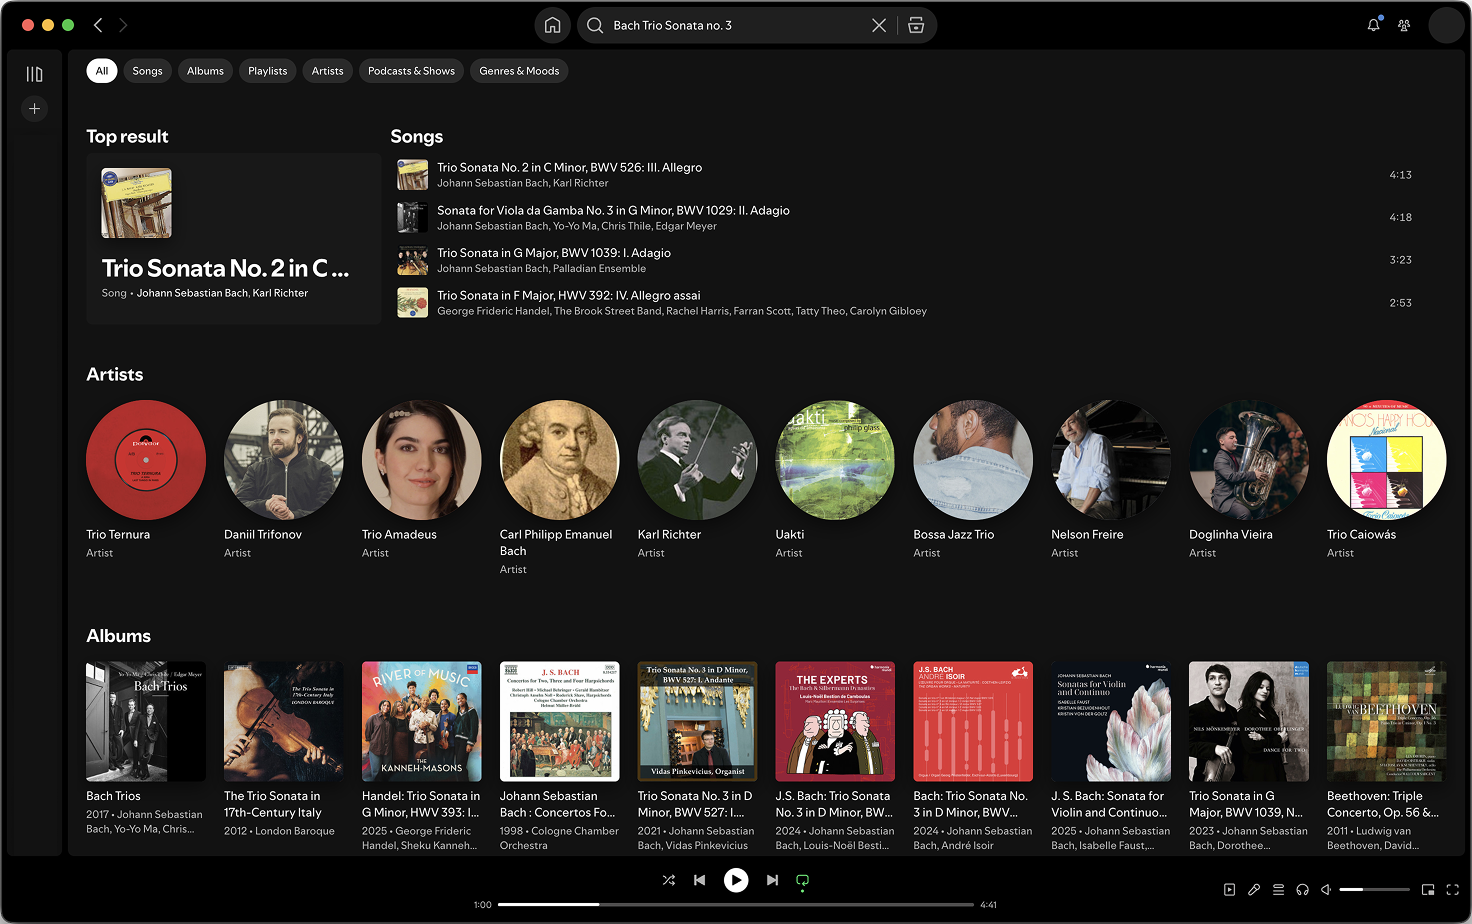
\includegraphics[width=1\textwidth]{figuras/Spotify.png}
\caption{Resultado de busca na plataforma Spotify}
\label{fig:spotify}
\end{figure}

Em contrapartida, existem plataformas de \emph{streaming} especializadas em
música clássica, como a plataforma IDAGIO e Presto Music, que adaptam seu
algoritmo de pesquisa especificamente para este nicho. Apesar disso, por se
tratar de um nicho limitado, há a grande iminência de um monopólio, por
existirem um número baixo de plataformas com funcionalidades voltadas para
ouvintes de música clássica. O principal exemplo desse movimento foi a aquisição
da antiga Primephonic pela Apple, criando a Apple Music Classical. Com isso,
abre-se o debate de se uma empresa privada com alcance de usuários diversificado
manteria a qualidade do serviço tendo em mente ser uma empresa privada que visa
primariamente o lucro, onde uma possível queda de ouvintes poderia tender a
abolição dessas funcionalidades e do desenvolvimento desse setor.

Por fim, este artigo cria uma implementação na seção seguinte de uma aplicação
computacional que visa democratizar o acesso de um algoritmo decente de busca
para música clássica, respeitando a necessidade explicitada anteriormente, por
meio de uma prova de conceito. Isso implica a liberdade de qualquer usuário
poder usar a solução de código livre disponibilizada podendo adaptar às próprias
necessidades, como o uso em plataformas de \emph{streaming} ou em arquivos
locais. Além disso, abre a possibilidade de empresas já estabelecidas no mercado
de criarem soluções embasadas para uma disponibilidade de funcionalidades mais
ampla dentre plataformas, desincentivando o monopólio da área.

\section{Implementação}

A implementação baseia-se na ideia de uma árvore de busca para o indexamento de
músicas clássicas, permitindo a obtenção de todas as gravações pelo termo de
busca, ou seja, o nome da composição. Para o desenvolvimento do sistema, foram
utilizadas duas alternativas de estruturas de dados semelhantes, as árvores B e
B\nolinebreak+ persistentes, permitindo que crie-se uma comparação direta entre
a eficiência em termos de complexidade de tempo, espaço e facilidade de
implementação.

Considerando a implementação, a estrutura de dados dentro das árvores B e
B\nolinebreak+ são usadas para guardar valores e registros. Com isso, o registro
guarda as seguintes informações:
\begin{itemize}
  \item Compositor (ex.: Ludwig van Beethoven);
  \item Nome da composição (ex.: Sinfonia no. 9);
  \item Catálogo (ex.: op. 125);
\end{itemize}

Além dessa estrutura, os metadados da música também compõem a própria chave,
sendo a chave composta como a concatenação do Compositor e do Catálogo (ex:
"Ludwig van Beethoven125"). Com isso, o principal valor de busca presente no
valor dos elementos da árvore é o nome da composição. Com isso, a árvore serve
como um indexamento de dados atrelados a um conjunto de gravações, cabendo o
acréscimo de informações de outros tipos de metadados, como duração média,
quantidade de gravações, etc.

Além disso, é criado dinâmicamente um arquivo único para cada composição que
contém uma listagem sequencial de todas as gravações dessa composição
analisadas. Esse arquivo é armazenado na memória secundária com o caminho
atrelado aos metadados armazenados na árvore. A decisão da sequencialidade do
arquivo digital justifica-se pelo objetivo final da listagem de todas as
gravações, simplificando a implementação do projeto.

Com a problemática em mente, foi decidida a implementação do programa utilizando
a linguagem C++, pois ela apresenta um conjunto de características
imprescindíveis para o projeto. A principal característica é sua alta
performance, provindo da sua natureza de compilação \emph{Ahead-of-Time} (AOT).
O quesito de tempo de execução é essencial para o projeto, já que o propósito é
uma ferramenta eficiente de busca. Outra característica da linguagem que
facilita a implementação é sua vasta quantidade de bibliotecas que incorporam
partes essenciais do código elaborado neste artigo.

As duas bibliotecas utilizadas foram o Tipo Abstrato de Dados (TAD) da árvore
B+\footnote{\url{https://github.com/ByJuanDiego/disk-b-plus-tree}} e a
biblioteca TagLib\footnote{\url{https://taglib.org/}}, para a leitura de
metadados de arquivos de música. Isso resultou numa implementação mais simples,
garantindo um código conciso e bem estruturado.

\section{Resultados}\label{sec:figs}
As árvores B e B\nolinebreak+ são úteis quando o conjunto de dados de consulta é
grande suficiente para não caber por completo na memória principal e precisa ser
acessado da memória secundária. Elas agem de maneira a buscar o menor número de
acessos ao disco para acessar efetivamente o registro requisitado. A altura
dessa estrutura de árvores está no intervalo de $[\log_{2t-1} (n+1),\ \log_t
\frac{n + 1}{2}]$, onde $t$ é a ordem da árvore que indica a quantidade mínima
de registros armazenados em um nó e $n$ a quantidade de elementos
\cite{clrs:22}. Com isso, a quantidade de acessos a páginas do disco é de
complexidade $O(\log_t n)$, entretanto, demora o tempo $O(t)$ para percorrer os
registros dentro de cada nó, compondo no final a complexidade de $O(t \log_t n)$
para buscas~\cite{clrs:22,Pm:10}. Por isso, são parte integrante da estrutura
central do projeto, pois permitem a indexação eficiente de cada composição a
partir de uma chave de identificação única, representado na
Tabela~\ref{tab:complexidades}.

\begin{table}[ht]
\centering
\caption{Tabela de Complexidades das Árvores B e B\nolinebreak+}
\label{tab:complexidades}
\begin{tabular}{|c|c|c|}
\hline
  Estrutura & Operação & Complexidade \\ \hline
  \multirow{4}{*}{Árvore B} & Espaço   & $O(n)$ \\
  \cline{2-3} & Busca    & $O(t \log_t n)$ \\
  \cline{2-3} & Inserção & $O(t \log_t n)$ \\
  \cline{2-3} & Remoção  & $O(t \log_t n)$ \\
  \hline
  \multirow{4}{*}{Árvore B\nolinebreak+} & Espaço & $O(n)$ \\
  \cline{2-3} & Busca & $O(t \log_t n)$ \\
  \cline{2-3} & Inserção & $O(t \log_t n)$\\
  \cline{2-3} & Remoção & $O(t \log_t n)$\\
  \hline
\end{tabular}
\end{table}


Figure and table captions should be centered if less than one line
(Figure~\ref{fig:exampleFig1}), otherwise justified and indented by 0.8cm on
both margins, as shown in Figure~\ref{fig:exampleFig2}. The caption font must be
Helvetica, 10 point, boldface, with 6 points of space before and after each
caption.

\begin{figure}[ht]
\centering
% \includegraphics[width=.5\textwidth]{fig1.jpg}
\caption{A typical figure}
\label{fig:exampleFig1}
\end{figure}

\begin{figure}[ht]
\centering
%\includegraphics[width=.3\textwidth]{fig2.jpg}
\caption{This figure is an example of a figure caption taking more than one line
  and justified considering margins mentioned in Section~\ref{sec:figs}.}
\label{fig:exampleFig2}
\end{figure}

In tables, try to avoid the use of colored or shaded backgrounds, and avoid
thick, doubled, or unnecessary framing lines. When reporting empirical data, do
not use more decimal digits than warranted by their precision and
reproducibility. Table caption must be placed before the table (see Table 1) and
the font used must also be Helvetica, 10 point, boldface, with 6 points of space
before and after each caption.

\begin{table}[ht]
\centering
\caption{Variables to be considered on the evaluation of interaction techniques}
\label{tab:exTable1}
% \includegraphics[width=.7\textwidth]{table.jpg}
\end{table}

\section{Conclusão}

All images and illustrations should be in black-and-white, or gray tones,
excepting for the papers that will be electronically available (on CD-ROMs,
internet, etc.). The image resolution on paper should be about 600 dpi for
black-and-white images, and 150-300 dpi for grayscale images.  Do not include
images with excessive resolution, as they may take hours to print, without any
visible difference in the result. 

\bibliographystyle{sbc}
\bibliography{bibliography}

\end{document}
